\def\pwidth{.32\linewidth}

\def\includeten#1#2{
\includegraphics[width=\pwidth]{#1ASW0007iwp_4XBJWT3COV#2}%
\includegraphics[width=\pwidth]{#1ASW0007xrs_JHC3J2HYV7#2}%
\includegraphics[width=\pwidth]{#1ASW0008pag_5SXGXQYY6V#2}\\
\includegraphics[width=\pwidth]{#1ASW0007k4r_N7LTELSYTM#2}%
\includegraphics[width=\pwidth]{#1ASW00096rm_4Q3YCEWGLN#2}%
\includegraphics[width=\pwidth]{#1ASW0001ld7_OS3CYAKLRT#2}\\
\includegraphics[width=\pwidth]{#1ASW0002asp_5EKMWWVJHL#2}%
\includegraphics[width=\pwidth]{#1ASW0008qsm_TOFS7JNGEK#2}%
\includegraphics[width=\pwidth]{#1ASW000619d_011489#2}\\
%\includegraphics[width=\pwidth]{#1ASW000096t_7IPP7LWVOF#2}%
}

\def\includezehn#1#2{
\includegraphics[width=\pwidth]{#1SW58_ASW0007iwp_4XBJWT3COV#2}%   L
\includegraphics[width=\pwidth]{#1SW28_ASW0007xrs_JHC3J2HYV7#2}%   L
\includegraphics[width=\pwidth]{#1SW57_ASW0008pag_5SXGXQYY6V#2}\\% X
\includegraphics[width=\pwidth]{#1SW05_ASW0007k4r_N7LTELSYTM#2}%   I
\includegraphics[width=\pwidth]{#1SW42_ASW00096rm_4Q3YCEWGLN#2}%   I
\includegraphics[width=\pwidth]{#1SW19_ASW0001ld7_OS3CYAKLRT#2}\\% I
\includegraphics[width=\pwidth]{#1SW09_ASW0002asp_5EKMWWVJHL#2}%   S
\includegraphics[width=\pwidth]{#1SW29_ASW0008qsm_TOFS7JNGEK#2}%   S
\includegraphics[width=\pwidth]{#1SW02_ASW000619d_011489#2}\\%     S
%\includegraphics[width=\pwidth]{#1SW36_ASW000096t_7IPP7LWVOF#2}%
}

\begin{figure*}
\includeten{spaghetti/}{_input}
\caption{Marked-up images. \label{fig:markedup}}
\end{figure*}

\begin{figure*}
\includezehn{img/arrival_spaghetti/}{_arrival_spaghetti}
\caption{\label{fig:arriv}}
\end{figure*}

\begin{figure*}
\includeten{img/nsynth/}{_nsynth}
\label{fig:synth}
\caption{}
\end{figure*}

\begin{figure*}
\includezehn{img/kappa_map/}{_kappa_map}
\caption{\label{fig:kappa}}
\end{figure*}

\begin{figure*}
\includezehn{img/kappa_encl/}{_kappa_encl}
\caption{}
\end{figure*}

\begin{figure*}
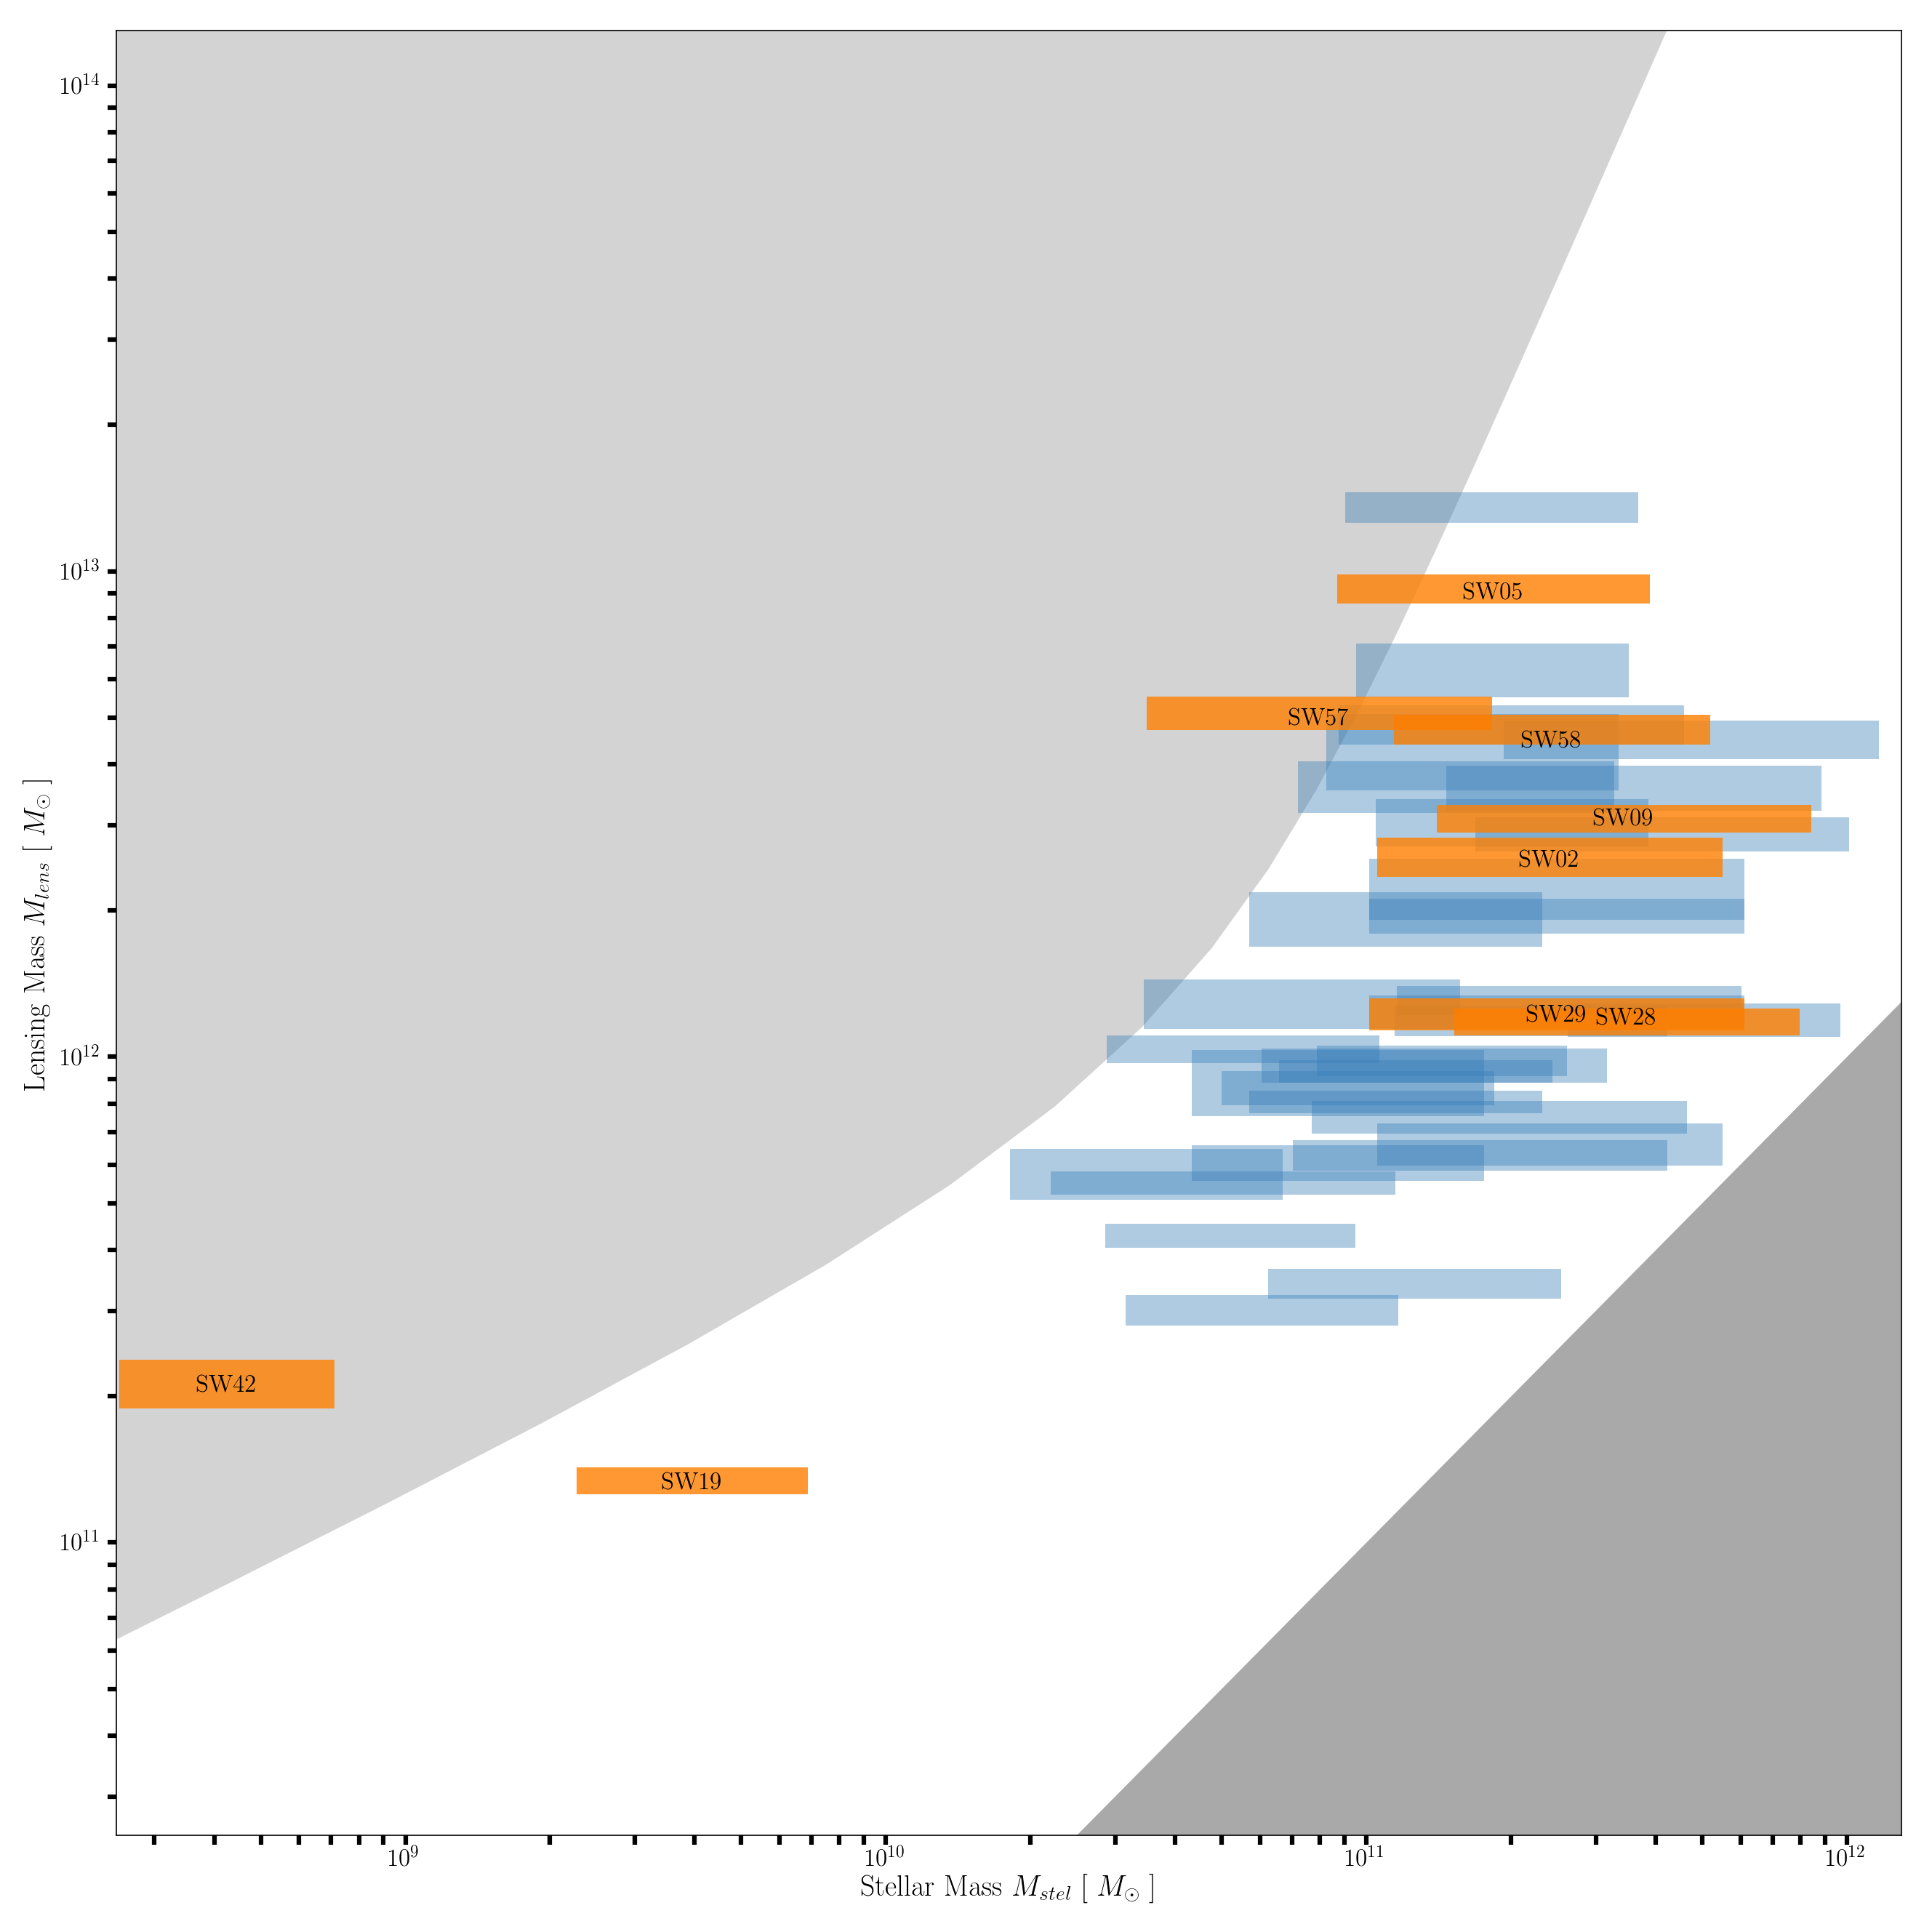
\includegraphics[width=\linewidth]{img/mlens_vs_mstel_one/mstel_vs_mtot_one}
\caption{Total mass in the model against the estimated stellar mass,
  alongside the values for the whole sample.  The lower-right shaded
  region is unphysical according to the stellar-population models,
  because it gives $M<\Mstel$. The upper-left shaded region is
  unphysical according to abundance matching, because it gives
  $M>\Mhalo$.  That is to say, the unshaded region is
  $0<\haloindex<1$. \label{fig:stelmass}}
\end{figure*}

